\documentclass[twoside]{book}

% Packages required by doxygen
\usepackage{fixltx2e}
\usepackage{calc}
\usepackage{doxygen}
\usepackage[export]{adjustbox} % also loads graphicx
\usepackage{graphicx}
\usepackage[utf8]{inputenc}
\usepackage{makeidx}
\usepackage{multicol}
\usepackage{multirow}
\PassOptionsToPackage{warn}{textcomp}
\usepackage{textcomp}
\usepackage[nointegrals]{wasysym}
\usepackage[table]{xcolor}

% NLS support packages
\usepackage[brazil]{babel}
% Font selection
\usepackage[T1]{fontenc}
\usepackage[scaled=.90]{helvet}
\usepackage{courier}
\usepackage{amssymb}
\usepackage{sectsty}
\renewcommand{\familydefault}{\sfdefault}
\allsectionsfont{%
  \fontseries{bc}\selectfont%
  \color{darkgray}%
}
\renewcommand{\DoxyLabelFont}{%
  \fontseries{bc}\selectfont%
  \color{darkgray}%
}
\newcommand{\+}{\discretionary{\mbox{\scriptsize$\hookleftarrow$}}{}{}}

% Page & text layout
\usepackage{geometry}
\geometry{%
  a4paper,%
  top=2.5cm,%
  bottom=2.5cm,%
  left=2.5cm,%
  right=2.5cm%
}
\tolerance=750
\hfuzz=15pt
\hbadness=750
\setlength{\emergencystretch}{15pt}
\setlength{\parindent}{0cm}
\setlength{\parskip}{3ex plus 2ex minus 2ex}
\makeatletter
\renewcommand{\paragraph}{%
  \@startsection{paragraph}{4}{0ex}{-1.0ex}{1.0ex}{%
    \normalfont\normalsize\bfseries\SS@parafont%
  }%
}
\renewcommand{\subparagraph}{%
  \@startsection{subparagraph}{5}{0ex}{-1.0ex}{1.0ex}{%
    \normalfont\normalsize\bfseries\SS@subparafont%
  }%
}
\makeatother

% Headers & footers
\usepackage{fancyhdr}
\pagestyle{fancyplain}
\fancyhead[LE]{\fancyplain{}{\bfseries\thepage}}
\fancyhead[CE]{\fancyplain{}{}}
\fancyhead[RE]{\fancyplain{}{\bfseries\leftmark}}
\fancyhead[LO]{\fancyplain{}{\bfseries\rightmark}}
\fancyhead[CO]{\fancyplain{}{}}
\fancyhead[RO]{\fancyplain{}{\bfseries\thepage}}
\fancyfoot[LE]{\fancyplain{}{}}
\fancyfoot[CE]{\fancyplain{}{}}
\fancyfoot[RE]{\fancyplain{}{\bfseries\scriptsize Gerado por Doxygen }}
\fancyfoot[LO]{\fancyplain{}{\bfseries\scriptsize Gerado por Doxygen }}
\fancyfoot[CO]{\fancyplain{}{}}
\fancyfoot[RO]{\fancyplain{}{}}
\renewcommand{\footrulewidth}{0.4pt}
\renewcommand{\chaptermark}[1]{%
  \markboth{#1}{}%
}
\renewcommand{\sectionmark}[1]{%
  \markright{\thesection\ #1}%
}

% Indices & bibliography
\usepackage{natbib}
\usepackage[titles]{tocloft}
\setcounter{tocdepth}{3}
\setcounter{secnumdepth}{5}
\makeindex

% Hyperlinks (required, but should be loaded last)
\usepackage{ifpdf}
\ifpdf
  \usepackage[pdftex,pagebackref=true]{hyperref}
\else
  \usepackage[ps2pdf,pagebackref=true]{hyperref}
\fi
\hypersetup{%
  colorlinks=true,%
  linkcolor=blue,%
  citecolor=blue,%
  unicode%
}

% Custom commands
\newcommand{\clearemptydoublepage}{%
  \newpage{\pagestyle{empty}\cleardoublepage}%
}

\usepackage{caption}
\captionsetup{labelsep=space,justification=centering,font={bf},singlelinecheck=off,skip=4pt,position=top}

%===== C O N T E N T S =====

\begin{document}

% Titlepage & ToC
\hypersetup{pageanchor=false,
             bookmarksnumbered=true,
             pdfencoding=unicode
            }
\pagenumbering{alph}
\begin{titlepage}
\vspace*{7cm}
\begin{center}%
{\Large Projeto P1 -\/ C\+C3642 \\[1ex]\large 1.\+0 }\\
\vspace*{1cm}
{\large Gerado por Doxygen 1.8.14}\\
\end{center}
\end{titlepage}
\clearemptydoublepage
\pagenumbering{roman}
\tableofcontents
\clearemptydoublepage
\pagenumbering{arabic}
\hypersetup{pageanchor=true}

%--- Begin generated contents ---
\chapter{Índice Hierárquico}
\section{Hierarquia de Classes}
Esta lista de hierarquias está parcialmente ordenada (ordem alfabética)\+:\begin{DoxyCompactList}
\item \contentsline{section}{Mundo}{\pageref{class_mundo}}{}
\item \contentsline{section}{Veiculo}{\pageref{class_veiculo}}{}
\begin{DoxyCompactList}
\item \contentsline{section}{Caminhao}{\pageref{class_caminhao}}{}
\item \contentsline{section}{Carro}{\pageref{class_carro}}{}
\item \contentsline{section}{Moto}{\pageref{class_moto}}{}
\end{DoxyCompactList}
\end{DoxyCompactList}

\chapter{Índice dos Componentes}
\section{Lista de Classes}
Aqui estão as classes, estruturas, uniões e interfaces e suas respectivas descrições\+:\begin{DoxyCompactList}
\item\contentsline{section}{\mbox{\hyperlink{class_caminhao}{Caminhao}} \\*Classe que representa um Caminhão; }{\pageref{class_caminhao}}{}
\item\contentsline{section}{\mbox{\hyperlink{class_carro}{Carro}} \\*Classe que representa um \mbox{\hyperlink{class_carro}{Carro}}; }{\pageref{class_carro}}{}
\item\contentsline{section}{\mbox{\hyperlink{class_moto}{Moto}} \\*Classe que representa uma \mbox{\hyperlink{class_moto}{Moto}}; }{\pageref{class_moto}}{}
\item\contentsline{section}{\mbox{\hyperlink{class_mundo}{Mundo}} \\*Classe que representa o mundo em que os veiculos se movem }{\pageref{class_mundo}}{}
\item\contentsline{section}{\mbox{\hyperlink{class_veiculo}{Veiculo}} \\*Classe com os atributos gerais de um \mbox{\hyperlink{class_veiculo}{Veiculo}}, serve de pai para veiculos especificos(motos, carros, etc...) }{\pageref{class_veiculo}}{}
\end{DoxyCompactList}

\chapter{Índice dos Arquivos}
\section{Lista de Arquivos}
Esta é a lista de todos os arquivos e suas respectivas descrições\+:\begin{DoxyCompactList}
\item\contentsline{section}{Projeto C\+C3642/\+App/\mbox{\hyperlink{_caminhao_8java}{Caminhao.\+java}} }{\pageref{_caminhao_8java}}{}
\item\contentsline{section}{Projeto C\+C3642/\+App/\mbox{\hyperlink{_carro_8java}{Carro.\+java}} }{\pageref{_carro_8java}}{}
\item\contentsline{section}{Projeto C\+C3642/\+App/\mbox{\hyperlink{_main_8java}{Main.\+java}} }{\pageref{_main_8java}}{}
\item\contentsline{section}{Projeto C\+C3642/\+App/\mbox{\hyperlink{_moto_8java}{Moto.\+java}} }{\pageref{_moto_8java}}{}
\item\contentsline{section}{Projeto C\+C3642/\+App/\mbox{\hyperlink{_mundo_8java}{Mundo.\+java}} }{\pageref{_mundo_8java}}{}
\item\contentsline{section}{Projeto C\+C3642/\+App/\mbox{\hyperlink{_veiculo_8java}{Veiculo.\+java}} }{\pageref{_veiculo_8java}}{}
\end{DoxyCompactList}

\chapter{Classes}
\hypertarget{class_caminhao}{}\section{Referência da Classe Caminhao}
\label{class_caminhao}\index{Caminhao@{Caminhao}}


Classe que representa um Caminhão;.  




Diagrama de hierarquia para Caminhao\+:
\nopagebreak
\begin{figure}[H]
\begin{center}
\leavevmode
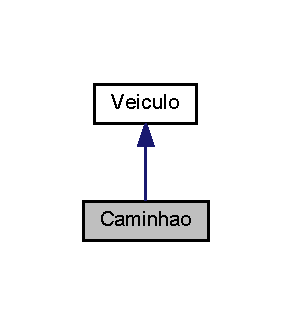
\includegraphics[width=140pt]{class_caminhao__inherit__graph}
\end{center}
\end{figure}


Diagrama de colaboração para Caminhao\+:
\nopagebreak
\begin{figure}[H]
\begin{center}
\leavevmode
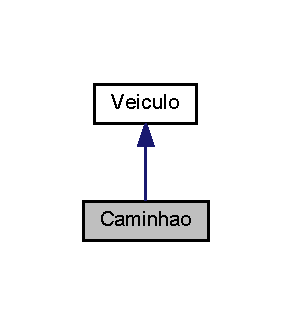
\includegraphics[width=140pt]{class_caminhao__coll__graph}
\end{center}
\end{figure}
\subsection*{Métodos Públicos}
\begin{DoxyCompactItemize}
\item 
\mbox{\hyperlink{class_caminhao_a7d012968951dc4bd2857c728dd3d0c79}{Caminhao}} (int \mbox{\hyperlink{class_veiculo_a069917a284297fe5b385258b2afd9ad6}{x}}, int \mbox{\hyperlink{class_veiculo_af25046404db7c2786c0d9e468bb1fb64}{y}})
\end{DoxyCompactItemize}
\subsection*{Atributos Privados}
\begin{DoxyCompactItemize}
\item 
int \mbox{\hyperlink{class_caminhao_a684d4c04ae732540eead2f735d221e7e}{capacidade\+\_\+carga}}
\begin{DoxyCompactList}\small\item\em Atributo para representar a quantidade de carga que o \mbox{\hyperlink{class_caminhao}{Caminhao}} suporta. \end{DoxyCompactList}\end{DoxyCompactItemize}
\subsection*{Outros membros herdados}


\subsection{Descrição detalhada}
Classe que representa um Caminhão;. 

\subsection{Construtores e Destrutores}
\mbox{\Hypertarget{class_caminhao_a7d012968951dc4bd2857c728dd3d0c79}\label{class_caminhao_a7d012968951dc4bd2857c728dd3d0c79}} 
\index{Caminhao@{Caminhao}!Caminhao@{Caminhao}}
\index{Caminhao@{Caminhao}!Caminhao@{Caminhao}}
\subsubsection{\texorpdfstring{Caminhao()}{Caminhao()}}
{\footnotesize\ttfamily Caminhao.\+Caminhao (\begin{DoxyParamCaption}\item[{int}]{x,  }\item[{int}]{y }\end{DoxyParamCaption})}

$<$ Construtor padrão que utiliza o contrutor padrão de veiculo e dá o valor 1 ao atributo velocidade. 

\subsection{Atributos}
\mbox{\Hypertarget{class_caminhao_a684d4c04ae732540eead2f735d221e7e}\label{class_caminhao_a684d4c04ae732540eead2f735d221e7e}} 
\index{Caminhao@{Caminhao}!capacidade\+\_\+carga@{capacidade\+\_\+carga}}
\index{capacidade\+\_\+carga@{capacidade\+\_\+carga}!Caminhao@{Caminhao}}
\subsubsection{\texorpdfstring{capacidade\+\_\+carga}{capacidade\_carga}}
{\footnotesize\ttfamily int Caminhao.\+capacidade\+\_\+carga\hspace{0.3cm}{\ttfamily [private]}}



Atributo para representar a quantidade de carga que o \mbox{\hyperlink{class_caminhao}{Caminhao}} suporta. 



A documentação para essa classe foi gerada a partir do seguinte arquivo\+:\begin{DoxyCompactItemize}
\item 
Projeto C\+C3642/\+App/\mbox{\hyperlink{_caminhao_8java}{Caminhao.\+java}}\end{DoxyCompactItemize}

\hypertarget{class_carro}{}\section{Referência da Classe Carro}
\label{class_carro}\index{Carro@{Carro}}


Classe que representa um \mbox{\hyperlink{class_carro}{Carro}};.  




Diagrama de hierarquia para Carro\+:
\nopagebreak
\begin{figure}[H]
\begin{center}
\leavevmode
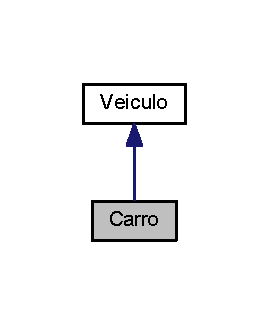
\includegraphics[width=129pt]{class_carro__inherit__graph}
\end{center}
\end{figure}


Diagrama de colaboração para Carro\+:
\nopagebreak
\begin{figure}[H]
\begin{center}
\leavevmode
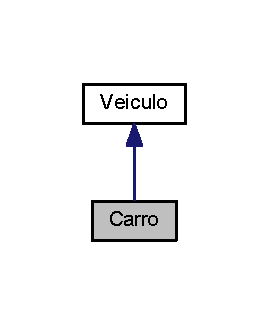
\includegraphics[width=129pt]{class_carro__coll__graph}
\end{center}
\end{figure}
\subsection*{Métodos Públicos}
\begin{DoxyCompactItemize}
\item 
\mbox{\hyperlink{class_carro_a52627c022471d194effbc51864c939c8}{Carro}} (int \mbox{\hyperlink{class_veiculo_a069917a284297fe5b385258b2afd9ad6}{x}}, int \mbox{\hyperlink{class_veiculo_af25046404db7c2786c0d9e468bb1fb64}{y}})
\end{DoxyCompactItemize}
\subsection*{Atributos Privados}
\begin{DoxyCompactItemize}
\item 
int \mbox{\hyperlink{class_carro_a60e3f3d344a7d3eebdf3104ff05de951}{num\+\_\+passageiros}}
\begin{DoxyCompactList}\small\item\em Atributo para representar o numero de passageiros que o carro suporta. \end{DoxyCompactList}\end{DoxyCompactItemize}
\subsection*{Outros membros herdados}


\subsection{Descrição detalhada}
Classe que representa um \mbox{\hyperlink{class_carro}{Carro}};. 

\subsection{Construtores e Destrutores}
\mbox{\Hypertarget{class_carro_a52627c022471d194effbc51864c939c8}\label{class_carro_a52627c022471d194effbc51864c939c8}} 
\index{Carro@{Carro}!Carro@{Carro}}
\index{Carro@{Carro}!Carro@{Carro}}
\subsubsection{\texorpdfstring{Carro()}{Carro()}}
{\footnotesize\ttfamily Carro.\+Carro (\begin{DoxyParamCaption}\item[{int}]{x,  }\item[{int}]{y }\end{DoxyParamCaption})}

$<$ Construtor padrão que utiliza o contrutor padrão de veiculo e dá o valor 2 ao atributo velocidade. 

\subsection{Atributos}
\mbox{\Hypertarget{class_carro_a60e3f3d344a7d3eebdf3104ff05de951}\label{class_carro_a60e3f3d344a7d3eebdf3104ff05de951}} 
\index{Carro@{Carro}!num\+\_\+passageiros@{num\+\_\+passageiros}}
\index{num\+\_\+passageiros@{num\+\_\+passageiros}!Carro@{Carro}}
\subsubsection{\texorpdfstring{num\+\_\+passageiros}{num\_passageiros}}
{\footnotesize\ttfamily int Carro.\+num\+\_\+passageiros\hspace{0.3cm}{\ttfamily [private]}}



Atributo para representar o numero de passageiros que o carro suporta. 



A documentação para essa classe foi gerada a partir do seguinte arquivo\+:\begin{DoxyCompactItemize}
\item 
Projeto C\+C3642/\+App/\mbox{\hyperlink{_carro_8java}{Carro.\+java}}\end{DoxyCompactItemize}

\hypertarget{class_moto}{}\section{Referência da Classe Moto}
\label{class_moto}\index{Moto@{Moto}}


Classe que representa uma \mbox{\hyperlink{class_moto}{Moto}};.  




Diagrama de hierarquia para Moto\+:
\nopagebreak
\begin{figure}[H]
\begin{center}
\leavevmode
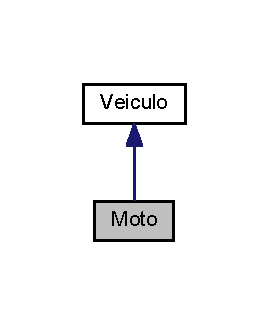
\includegraphics[width=129pt]{class_moto__inherit__graph}
\end{center}
\end{figure}


Diagrama de colaboração para Moto\+:
\nopagebreak
\begin{figure}[H]
\begin{center}
\leavevmode
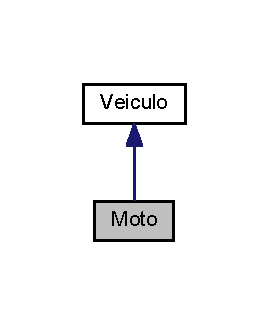
\includegraphics[width=129pt]{class_moto__coll__graph}
\end{center}
\end{figure}
\subsection*{Métodos Públicos}
\begin{DoxyCompactItemize}
\item 
\mbox{\hyperlink{class_moto_a803d5eb919bb5e4c6f30e5455cf28097}{Moto}} (int \mbox{\hyperlink{class_veiculo_a069917a284297fe5b385258b2afd9ad6}{x}}, int \mbox{\hyperlink{class_veiculo_af25046404db7c2786c0d9e468bb1fb64}{y}})
\end{DoxyCompactItemize}
\subsection*{Atributos Privados}
\begin{DoxyCompactItemize}
\item 
String \mbox{\hyperlink{class_moto_a98533b801c6277bdac415e9d21f74efe}{tipo}}
\begin{DoxyCompactList}\small\item\em Atributo para representar o tipo de moto. \end{DoxyCompactList}\end{DoxyCompactItemize}
\subsection*{Outros membros herdados}


\subsection{Descrição detalhada}
Classe que representa uma \mbox{\hyperlink{class_moto}{Moto}};. 

\subsection{Construtores e Destrutores}
\mbox{\Hypertarget{class_moto_a803d5eb919bb5e4c6f30e5455cf28097}\label{class_moto_a803d5eb919bb5e4c6f30e5455cf28097}} 
\index{Moto@{Moto}!Moto@{Moto}}
\index{Moto@{Moto}!Moto@{Moto}}
\subsubsection{\texorpdfstring{Moto()}{Moto()}}
{\footnotesize\ttfamily Moto.\+Moto (\begin{DoxyParamCaption}\item[{int}]{x,  }\item[{int}]{y }\end{DoxyParamCaption})}

$<$ Construtor padrão que utiliza o contrutor padrão de veiculo e dá o valor 3 ao atributo velocidade. 

\subsection{Atributos}
\mbox{\Hypertarget{class_moto_a98533b801c6277bdac415e9d21f74efe}\label{class_moto_a98533b801c6277bdac415e9d21f74efe}} 
\index{Moto@{Moto}!tipo@{tipo}}
\index{tipo@{tipo}!Moto@{Moto}}
\subsubsection{\texorpdfstring{tipo}{tipo}}
{\footnotesize\ttfamily String Moto.\+tipo\hspace{0.3cm}{\ttfamily [private]}}



Atributo para representar o tipo de moto. 



A documentação para essa classe foi gerada a partir do seguinte arquivo\+:\begin{DoxyCompactItemize}
\item 
Projeto C\+C3642/\+App/\mbox{\hyperlink{_moto_8java}{Moto.\+java}}\end{DoxyCompactItemize}

\hypertarget{class_mundo}{}\section{Referência da Classe Mundo}
\label{class_mundo}\index{Mundo@{Mundo}}


Classe que representa o mundo em que os veiculos se movem.  


\subsection*{Métodos Públicos}
\begin{DoxyCompactItemize}
\item 
void \mbox{\hyperlink{class_mundo_a89da5526d6fa79801cfa48b587aa8343}{cria\+Mundo}} (Array\+List$<$ \mbox{\hyperlink{class_moto}{Moto}} $>$ mot, Array\+List$<$ \mbox{\hyperlink{class_carro}{Carro}} $>$ car, Array\+List$<$ \mbox{\hyperlink{class_caminhao}{Caminhao}} $>$ cam)
\item 
void \mbox{\hyperlink{class_mundo_aaf8ab7632e91cf6b92d8beb031858de1}{check\+Fab}} (Array\+List$<$ \mbox{\hyperlink{class_moto}{Moto}} $>$ mot, Array\+List$<$ \mbox{\hyperlink{class_carro}{Carro}} $>$ car, Array\+List$<$ \mbox{\hyperlink{class_caminhao}{Caminhao}} $>$ cam)
\item 
void \mbox{\hyperlink{class_mundo_a0317827fd7dc86705d5ad3fb86d61741}{check\+Del}} (Array\+List$<$ \mbox{\hyperlink{class_moto}{Moto}} $>$ mot, Array\+List$<$ \mbox{\hyperlink{class_carro}{Carro}} $>$ car, Array\+List$<$ \mbox{\hyperlink{class_caminhao}{Caminhao}} $>$ cam)
\item 
void \mbox{\hyperlink{class_mundo_a7c0f57fc41e5712a905bc836c9d1f9c5}{con\+Int2\+Str}} ()
\item 
void \mbox{\hyperlink{class_mundo_a52455726daee2575ad03b11441fea89e}{imprime\+MundoS}} (Array\+List$<$ \mbox{\hyperlink{class_moto}{Moto}} $>$ mot, Array\+List$<$ \mbox{\hyperlink{class_carro}{Carro}} $>$ car, Array\+List$<$ \mbox{\hyperlink{class_caminhao}{Caminhao}} $>$ cam)
\end{DoxyCompactItemize}
\subsection*{Atributos Públicos}
\begin{DoxyCompactItemize}
\item 
int \mbox{\hyperlink{class_mundo_a8332b2d52b9f317338a4d6cbe10bbcbb}{mapa}} \mbox{[}$\,$\mbox{]}\mbox{[}$\,$\mbox{]} = new int\mbox{[}30\mbox{]}\mbox{[}60\mbox{]}
\begin{DoxyCompactList}\small\item\em Atributo para representar o mundo em forma de inteiros. \end{DoxyCompactList}\item 
String \mbox{\hyperlink{class_mundo_ac3b4e49cf251690a1ad421b3e8458ec6}{MapaS}} \mbox{[}$\,$\mbox{]}\mbox{[}$\,$\mbox{]} = new String\mbox{[}30\mbox{]}\mbox{[}60\mbox{]}
\begin{DoxyCompactList}\small\item\em Atributo para representar o mundo em forma de String(melhor visualização). \end{DoxyCompactList}\end{DoxyCompactItemize}


\subsection{Descrição detalhada}
Classe que representa o mundo em que os veiculos se movem. 

\subsection{Métodos}
\mbox{\Hypertarget{class_mundo_a0317827fd7dc86705d5ad3fb86d61741}\label{class_mundo_a0317827fd7dc86705d5ad3fb86d61741}} 
\index{Mundo@{Mundo}!check\+Del@{check\+Del}}
\index{check\+Del@{check\+Del}!Mundo@{Mundo}}
\subsubsection{\texorpdfstring{check\+Del()}{checkDel()}}
{\footnotesize\ttfamily void Mundo.\+check\+Del (\begin{DoxyParamCaption}\item[{Array\+List$<$ \mbox{\hyperlink{class_moto}{Moto}} $>$}]{mot,  }\item[{Array\+List$<$ \mbox{\hyperlink{class_carro}{Carro}} $>$}]{car,  }\item[{Array\+List$<$ \mbox{\hyperlink{class_caminhao}{Caminhao}} $>$}]{cam }\end{DoxyParamCaption})}

$<$ Método que verifica as posições dos veiculos, se estiverem, remove o que tem menor velocidade do mapa, se tiverem velocidade igual, remove os dois. \mbox{\Hypertarget{class_mundo_aaf8ab7632e91cf6b92d8beb031858de1}\label{class_mundo_aaf8ab7632e91cf6b92d8beb031858de1}} 
\index{Mundo@{Mundo}!check\+Fab@{check\+Fab}}
\index{check\+Fab@{check\+Fab}!Mundo@{Mundo}}
\subsubsection{\texorpdfstring{check\+Fab()}{checkFab()}}
{\footnotesize\ttfamily void Mundo.\+check\+Fab (\begin{DoxyParamCaption}\item[{Array\+List$<$ \mbox{\hyperlink{class_moto}{Moto}} $>$}]{mot,  }\item[{Array\+List$<$ \mbox{\hyperlink{class_carro}{Carro}} $>$}]{car,  }\item[{Array\+List$<$ \mbox{\hyperlink{class_caminhao}{Caminhao}} $>$}]{cam }\end{DoxyParamCaption})}

$<$ Método que verifica se o veiculo está sobre uma fabrica, se sim, gera o veiculo em cima dela. \mbox{\Hypertarget{class_mundo_a7c0f57fc41e5712a905bc836c9d1f9c5}\label{class_mundo_a7c0f57fc41e5712a905bc836c9d1f9c5}} 
\index{Mundo@{Mundo}!con\+Int2\+Str@{con\+Int2\+Str}}
\index{con\+Int2\+Str@{con\+Int2\+Str}!Mundo@{Mundo}}
\subsubsection{\texorpdfstring{con\+Int2\+Str()}{conInt2Str()}}
{\footnotesize\ttfamily void Mundo.\+con\+Int2\+Str (\begin{DoxyParamCaption}{ }\end{DoxyParamCaption})}

$<$ Método que gera um mapa no formato string apartir do mapa no formato de inteiros. \mbox{\Hypertarget{class_mundo_a89da5526d6fa79801cfa48b587aa8343}\label{class_mundo_a89da5526d6fa79801cfa48b587aa8343}} 
\index{Mundo@{Mundo}!cria\+Mundo@{cria\+Mundo}}
\index{cria\+Mundo@{cria\+Mundo}!Mundo@{Mundo}}
\subsubsection{\texorpdfstring{cria\+Mundo()}{criaMundo()}}
{\footnotesize\ttfamily void Mundo.\+cria\+Mundo (\begin{DoxyParamCaption}\item[{Array\+List$<$ \mbox{\hyperlink{class_moto}{Moto}} $>$}]{mot,  }\item[{Array\+List$<$ \mbox{\hyperlink{class_carro}{Carro}} $>$}]{car,  }\item[{Array\+List$<$ \mbox{\hyperlink{class_caminhao}{Caminhao}} $>$}]{cam }\end{DoxyParamCaption})}

$<$Método que cria o mapa com os veiculos nele. \mbox{\Hypertarget{class_mundo_a52455726daee2575ad03b11441fea89e}\label{class_mundo_a52455726daee2575ad03b11441fea89e}} 
\index{Mundo@{Mundo}!imprime\+MundoS@{imprime\+MundoS}}
\index{imprime\+MundoS@{imprime\+MundoS}!Mundo@{Mundo}}
\subsubsection{\texorpdfstring{imprime\+Mundo\+S()}{imprimeMundoS()}}
{\footnotesize\ttfamily void Mundo.\+imprime\+MundoS (\begin{DoxyParamCaption}\item[{Array\+List$<$ \mbox{\hyperlink{class_moto}{Moto}} $>$}]{mot,  }\item[{Array\+List$<$ \mbox{\hyperlink{class_carro}{Carro}} $>$}]{car,  }\item[{Array\+List$<$ \mbox{\hyperlink{class_caminhao}{Caminhao}} $>$}]{cam }\end{DoxyParamCaption})}

$<$ Método que imprime o mapa no formato de string. 

\subsection{Atributos}
\mbox{\Hypertarget{class_mundo_a8332b2d52b9f317338a4d6cbe10bbcbb}\label{class_mundo_a8332b2d52b9f317338a4d6cbe10bbcbb}} 
\index{Mundo@{Mundo}!mapa@{mapa}}
\index{mapa@{mapa}!Mundo@{Mundo}}
\subsubsection{\texorpdfstring{mapa}{mapa}}
{\footnotesize\ttfamily int Mundo.\+mapa\mbox{[}$\,$\mbox{]}\mbox{[}$\,$\mbox{]} = new int\mbox{[}30\mbox{]}\mbox{[}60\mbox{]}}



Atributo para representar o mundo em forma de inteiros. 

\mbox{\Hypertarget{class_mundo_ac3b4e49cf251690a1ad421b3e8458ec6}\label{class_mundo_ac3b4e49cf251690a1ad421b3e8458ec6}} 
\index{Mundo@{Mundo}!MapaS@{MapaS}}
\index{MapaS@{MapaS}!Mundo@{Mundo}}
\subsubsection{\texorpdfstring{MapaS}{MapaS}}
{\footnotesize\ttfamily String Mundo.\+MapaS\mbox{[}$\,$\mbox{]}\mbox{[}$\,$\mbox{]} = new String\mbox{[}30\mbox{]}\mbox{[}60\mbox{]}}



Atributo para representar o mundo em forma de String(melhor visualização). 



A documentação para essa classe foi gerada a partir do seguinte arquivo\+:\begin{DoxyCompactItemize}
\item 
Projeto C\+C3642/\+App/\mbox{\hyperlink{_mundo_8java}{Mundo.\+java}}\end{DoxyCompactItemize}

\hypertarget{class_veiculo}{}\section{Referência da Classe Veiculo}
\label{class_veiculo}\index{Veiculo@{Veiculo}}


Classe com os atributos gerais de um \mbox{\hyperlink{class_veiculo}{Veiculo}}, serve de pai para veiculos especificos(motos, carros, etc...).  




Diagrama de hierarquia para Veiculo\+:
\nopagebreak
\begin{figure}[H]
\begin{center}
\leavevmode
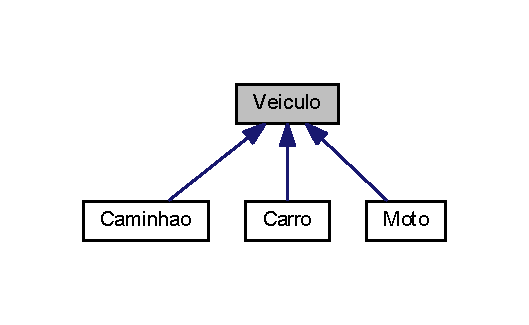
\includegraphics[width=254pt]{class_veiculo__inherit__graph}
\end{center}
\end{figure}
\subsection*{Métodos Públicos}
\begin{DoxyCompactItemize}
\item 
\mbox{\hyperlink{class_veiculo_a47f634662187ef78027f99a3ab6708a5}{Veiculo}} (int \mbox{\hyperlink{class_veiculo_a069917a284297fe5b385258b2afd9ad6}{x}}, int \mbox{\hyperlink{class_veiculo_af25046404db7c2786c0d9e468bb1fb64}{y}})
\item 
void \mbox{\hyperlink{class_veiculo_a3341b0ed6b4d34db990a31f7a499ae80}{move}} ()
\item 
void \mbox{\hyperlink{class_veiculo_af565d4a9368f62efe67608dbcf18ef2d}{check\+Fab}} ()
\item 
void \mbox{\hyperlink{class_veiculo_a84b2207a013e6cd869959b73a93864b8}{setX}} (int \mbox{\hyperlink{class_veiculo_a069917a284297fe5b385258b2afd9ad6}{x}})
\item 
void \mbox{\hyperlink{class_veiculo_a6d69355a635fa5c8d40ec87e3d6f9c10}{set\+Vel}} (int vel)
\item 
void \mbox{\hyperlink{class_veiculo_a57cb54424b47643d8b388c72dbaf43b1}{setY}} (int \mbox{\hyperlink{class_veiculo_af25046404db7c2786c0d9e468bb1fb64}{y}})
\item 
int \mbox{\hyperlink{class_veiculo_a235b29e1e25ec8c769b20fb2aeba8404}{getX}} ()
\item 
int \mbox{\hyperlink{class_veiculo_ab43d327b067e15c1bc96cee94d495049}{get\+Vel}} ()
\item 
int \mbox{\hyperlink{class_veiculo_a06b2a923e51186673a016f75d10363d3}{getY}} ()
\item 
boolean \mbox{\hyperlink{class_veiculo_a7509d7e1ba79a662b145f8907c4e97c1}{get\+Fab}} ()
\item 
void \mbox{\hyperlink{class_veiculo_af740c4bac90ecf0936dbdab300cf5776}{set\+Fab}} (boolean fab)
\end{DoxyCompactItemize}
\subsection*{Atributos Protegidos}
\begin{DoxyCompactItemize}
\item 
int \mbox{\hyperlink{class_veiculo_a2edf5e3132b1c2504c441dc095dc7e0e}{velocidade}}
\begin{DoxyCompactList}\small\item\em Atributo que representa a velocidade que o veiculo se movimenta no mapa. \end{DoxyCompactList}\item 
boolean \mbox{\hyperlink{class_veiculo_a23d377a69bdf558ebedb5bc35dcdebf5}{fabrica}}
\begin{DoxyCompactList}\small\item\em Atributo que representa se o veiculo está em cima de uma fábrica. \end{DoxyCompactList}\end{DoxyCompactItemize}
\subsection*{Atributos Privados}
\begin{DoxyCompactItemize}
\item 
int \mbox{\hyperlink{class_veiculo_af25046404db7c2786c0d9e468bb1fb64}{y}}
\begin{DoxyCompactList}\small\item\em Atributo que representa o eixo y do veiculo no mapa. \end{DoxyCompactList}\item 
int \mbox{\hyperlink{class_veiculo_a069917a284297fe5b385258b2afd9ad6}{x}}
\begin{DoxyCompactList}\small\item\em Atributo que representa o eixo x do veiculo no mapa. \end{DoxyCompactList}\item 
String \mbox{\hyperlink{class_veiculo_a6bc5886e61340672e69bd638936ec1d5}{cor}}
\begin{DoxyCompactList}\small\item\em Atributo que representa a cor do veiculo. \end{DoxyCompactList}\end{DoxyCompactItemize}


\subsection{Descrição detalhada}
Classe com os atributos gerais de um \mbox{\hyperlink{class_veiculo}{Veiculo}}, serve de pai para veiculos especificos(motos, carros, etc...). 

\subsection{Construtores e Destrutores}
\mbox{\Hypertarget{class_veiculo_a47f634662187ef78027f99a3ab6708a5}\label{class_veiculo_a47f634662187ef78027f99a3ab6708a5}} 
\index{Veiculo@{Veiculo}!Veiculo@{Veiculo}}
\index{Veiculo@{Veiculo}!Veiculo@{Veiculo}}
\subsubsection{\texorpdfstring{Veiculo()}{Veiculo()}}
{\footnotesize\ttfamily Veiculo.\+Veiculo (\begin{DoxyParamCaption}\item[{int}]{x,  }\item[{int}]{y }\end{DoxyParamCaption})}

$<$ Método utilizado como construtor padrão. 

\subsection{Métodos}
\mbox{\Hypertarget{class_veiculo_af565d4a9368f62efe67608dbcf18ef2d}\label{class_veiculo_af565d4a9368f62efe67608dbcf18ef2d}} 
\index{Veiculo@{Veiculo}!check\+Fab@{check\+Fab}}
\index{check\+Fab@{check\+Fab}!Veiculo@{Veiculo}}
\subsubsection{\texorpdfstring{check\+Fab()}{checkFab()}}
{\footnotesize\ttfamily void Veiculo.\+check\+Fab (\begin{DoxyParamCaption}{ }\end{DoxyParamCaption})}

$<$ Método que verifica se o veiculo está sobre uma fábrica, se estiver, muda o booleano fabrica pra true. \mbox{\Hypertarget{class_veiculo_a7509d7e1ba79a662b145f8907c4e97c1}\label{class_veiculo_a7509d7e1ba79a662b145f8907c4e97c1}} 
\index{Veiculo@{Veiculo}!get\+Fab@{get\+Fab}}
\index{get\+Fab@{get\+Fab}!Veiculo@{Veiculo}}
\subsubsection{\texorpdfstring{get\+Fab()}{getFab()}}
{\footnotesize\ttfamily boolean Veiculo.\+get\+Fab (\begin{DoxyParamCaption}{ }\end{DoxyParamCaption})}

$<$ Método get do atributo fabrica \mbox{\Hypertarget{class_veiculo_ab43d327b067e15c1bc96cee94d495049}\label{class_veiculo_ab43d327b067e15c1bc96cee94d495049}} 
\index{Veiculo@{Veiculo}!get\+Vel@{get\+Vel}}
\index{get\+Vel@{get\+Vel}!Veiculo@{Veiculo}}
\subsubsection{\texorpdfstring{get\+Vel()}{getVel()}}
{\footnotesize\ttfamily int Veiculo.\+get\+Vel (\begin{DoxyParamCaption}{ }\end{DoxyParamCaption})}

$<$ Método get do atributo velocidade \mbox{\Hypertarget{class_veiculo_a235b29e1e25ec8c769b20fb2aeba8404}\label{class_veiculo_a235b29e1e25ec8c769b20fb2aeba8404}} 
\index{Veiculo@{Veiculo}!getX@{getX}}
\index{getX@{getX}!Veiculo@{Veiculo}}
\subsubsection{\texorpdfstring{get\+X()}{getX()}}
{\footnotesize\ttfamily int Veiculo.\+getX (\begin{DoxyParamCaption}{ }\end{DoxyParamCaption})}

$<$ Método get do atributo x \mbox{\Hypertarget{class_veiculo_a06b2a923e51186673a016f75d10363d3}\label{class_veiculo_a06b2a923e51186673a016f75d10363d3}} 
\index{Veiculo@{Veiculo}!getY@{getY}}
\index{getY@{getY}!Veiculo@{Veiculo}}
\subsubsection{\texorpdfstring{get\+Y()}{getY()}}
{\footnotesize\ttfamily int Veiculo.\+getY (\begin{DoxyParamCaption}{ }\end{DoxyParamCaption})}

$<$ Método get do atributo y \mbox{\Hypertarget{class_veiculo_a3341b0ed6b4d34db990a31f7a499ae80}\label{class_veiculo_a3341b0ed6b4d34db990a31f7a499ae80}} 
\index{Veiculo@{Veiculo}!move@{move}}
\index{move@{move}!Veiculo@{Veiculo}}
\subsubsection{\texorpdfstring{move()}{move()}}
{\footnotesize\ttfamily void Veiculo.\+move (\begin{DoxyParamCaption}{ }\end{DoxyParamCaption})}

$<$ Método que move os veiculos. \mbox{\Hypertarget{class_veiculo_af740c4bac90ecf0936dbdab300cf5776}\label{class_veiculo_af740c4bac90ecf0936dbdab300cf5776}} 
\index{Veiculo@{Veiculo}!set\+Fab@{set\+Fab}}
\index{set\+Fab@{set\+Fab}!Veiculo@{Veiculo}}
\subsubsection{\texorpdfstring{set\+Fab()}{setFab()}}
{\footnotesize\ttfamily void Veiculo.\+set\+Fab (\begin{DoxyParamCaption}\item[{boolean}]{fab }\end{DoxyParamCaption})}

$<$ Método get do atributo fabrica \mbox{\Hypertarget{class_veiculo_a6d69355a635fa5c8d40ec87e3d6f9c10}\label{class_veiculo_a6d69355a635fa5c8d40ec87e3d6f9c10}} 
\index{Veiculo@{Veiculo}!set\+Vel@{set\+Vel}}
\index{set\+Vel@{set\+Vel}!Veiculo@{Veiculo}}
\subsubsection{\texorpdfstring{set\+Vel()}{setVel()}}
{\footnotesize\ttfamily void Veiculo.\+set\+Vel (\begin{DoxyParamCaption}\item[{int}]{vel }\end{DoxyParamCaption})}

$<$ Método set do atributo velocidade \mbox{\Hypertarget{class_veiculo_a84b2207a013e6cd869959b73a93864b8}\label{class_veiculo_a84b2207a013e6cd869959b73a93864b8}} 
\index{Veiculo@{Veiculo}!setX@{setX}}
\index{setX@{setX}!Veiculo@{Veiculo}}
\subsubsection{\texorpdfstring{set\+X()}{setX()}}
{\footnotesize\ttfamily void Veiculo.\+setX (\begin{DoxyParamCaption}\item[{int}]{x }\end{DoxyParamCaption})}

$<$ Método set do atributo x \mbox{\Hypertarget{class_veiculo_a57cb54424b47643d8b388c72dbaf43b1}\label{class_veiculo_a57cb54424b47643d8b388c72dbaf43b1}} 
\index{Veiculo@{Veiculo}!setY@{setY}}
\index{setY@{setY}!Veiculo@{Veiculo}}
\subsubsection{\texorpdfstring{set\+Y()}{setY()}}
{\footnotesize\ttfamily void Veiculo.\+setY (\begin{DoxyParamCaption}\item[{int}]{y }\end{DoxyParamCaption})}

$<$ Método set do atributo y 

\subsection{Atributos}
\mbox{\Hypertarget{class_veiculo_a6bc5886e61340672e69bd638936ec1d5}\label{class_veiculo_a6bc5886e61340672e69bd638936ec1d5}} 
\index{Veiculo@{Veiculo}!cor@{cor}}
\index{cor@{cor}!Veiculo@{Veiculo}}
\subsubsection{\texorpdfstring{cor}{cor}}
{\footnotesize\ttfamily String Veiculo.\+cor\hspace{0.3cm}{\ttfamily [private]}}



Atributo que representa a cor do veiculo. 

\mbox{\Hypertarget{class_veiculo_a23d377a69bdf558ebedb5bc35dcdebf5}\label{class_veiculo_a23d377a69bdf558ebedb5bc35dcdebf5}} 
\index{Veiculo@{Veiculo}!fabrica@{fabrica}}
\index{fabrica@{fabrica}!Veiculo@{Veiculo}}
\subsubsection{\texorpdfstring{fabrica}{fabrica}}
{\footnotesize\ttfamily boolean Veiculo.\+fabrica\hspace{0.3cm}{\ttfamily [protected]}}



Atributo que representa se o veiculo está em cima de uma fábrica. 

\mbox{\Hypertarget{class_veiculo_a2edf5e3132b1c2504c441dc095dc7e0e}\label{class_veiculo_a2edf5e3132b1c2504c441dc095dc7e0e}} 
\index{Veiculo@{Veiculo}!velocidade@{velocidade}}
\index{velocidade@{velocidade}!Veiculo@{Veiculo}}
\subsubsection{\texorpdfstring{velocidade}{velocidade}}
{\footnotesize\ttfamily int Veiculo.\+velocidade\hspace{0.3cm}{\ttfamily [protected]}}



Atributo que representa a velocidade que o veiculo se movimenta no mapa. 

\mbox{\Hypertarget{class_veiculo_a069917a284297fe5b385258b2afd9ad6}\label{class_veiculo_a069917a284297fe5b385258b2afd9ad6}} 
\index{Veiculo@{Veiculo}!x@{x}}
\index{x@{x}!Veiculo@{Veiculo}}
\subsubsection{\texorpdfstring{x}{x}}
{\footnotesize\ttfamily int Veiculo.\+x\hspace{0.3cm}{\ttfamily [private]}}



Atributo que representa o eixo x do veiculo no mapa. 

\mbox{\Hypertarget{class_veiculo_af25046404db7c2786c0d9e468bb1fb64}\label{class_veiculo_af25046404db7c2786c0d9e468bb1fb64}} 
\index{Veiculo@{Veiculo}!y@{y}}
\index{y@{y}!Veiculo@{Veiculo}}
\subsubsection{\texorpdfstring{y}{y}}
{\footnotesize\ttfamily int Veiculo.\+y\hspace{0.3cm}{\ttfamily [private]}}



Atributo que representa o eixo y do veiculo no mapa. 



A documentação para essa classe foi gerada a partir do seguinte arquivo\+:\begin{DoxyCompactItemize}
\item 
Projeto C\+C3642/\+App/\mbox{\hyperlink{_veiculo_8java}{Veiculo.\+java}}\end{DoxyCompactItemize}

\chapter{Arquivos}
\hypertarget{_caminhao_8java}{}\section{Referência do Arquivo Projeto C\+C3642/\+App/\+Caminhao.java}
\label{_caminhao_8java}\index{Projeto C\+C3642/\+App/\+Caminhao.\+java@{Projeto C\+C3642/\+App/\+Caminhao.\+java}}
\subsection*{Componentes}
\begin{DoxyCompactItemize}
\item 
class \mbox{\hyperlink{class_caminhao}{Caminhao}}
\begin{DoxyCompactList}\small\item\em Classe que representa um Caminhão;. \end{DoxyCompactList}\end{DoxyCompactItemize}

\hypertarget{_carro_8java}{}\section{Referência do Arquivo Projeto C\+C3642/\+App/\+Carro.java}
\label{_carro_8java}\index{Projeto C\+C3642/\+App/\+Carro.\+java@{Projeto C\+C3642/\+App/\+Carro.\+java}}
\subsection*{Componentes}
\begin{DoxyCompactItemize}
\item 
class \mbox{\hyperlink{class_carro}{Carro}}
\begin{DoxyCompactList}\small\item\em Classe que representa um \mbox{\hyperlink{class_carro}{Carro}};. \end{DoxyCompactList}\end{DoxyCompactItemize}

\hypertarget{_main_8java}{}\section{Referência do Arquivo Projeto C\+C3642/\+App/\+Main.java}
\label{_main_8java}\index{Projeto C\+C3642/\+App/\+Main.\+java@{Projeto C\+C3642/\+App/\+Main.\+java}}

\hypertarget{_moto_8java}{}\section{Referência do Arquivo Projeto C\+C3642/\+App/\+Moto.java}
\label{_moto_8java}\index{Projeto C\+C3642/\+App/\+Moto.\+java@{Projeto C\+C3642/\+App/\+Moto.\+java}}
\subsection*{Componentes}
\begin{DoxyCompactItemize}
\item 
class \mbox{\hyperlink{class_moto}{Moto}}
\begin{DoxyCompactList}\small\item\em Classe que representa uma \mbox{\hyperlink{class_moto}{Moto}};. \end{DoxyCompactList}\end{DoxyCompactItemize}

\hypertarget{_mundo_8java}{}\section{Referência do Arquivo Projeto C\+C3642/\+App/\+Mundo.java}
\label{_mundo_8java}\index{Projeto C\+C3642/\+App/\+Mundo.\+java@{Projeto C\+C3642/\+App/\+Mundo.\+java}}
\subsection*{Componentes}
\begin{DoxyCompactItemize}
\item 
class \mbox{\hyperlink{class_mundo}{Mundo}}
\begin{DoxyCompactList}\small\item\em Classe que representa o mundo em que os veiculos se movem. \end{DoxyCompactList}\end{DoxyCompactItemize}

\hypertarget{_veiculo_8java}{}\section{Referência do Arquivo Projeto C\+C3642/\+App/\+Veiculo.java}
\label{_veiculo_8java}\index{Projeto C\+C3642/\+App/\+Veiculo.\+java@{Projeto C\+C3642/\+App/\+Veiculo.\+java}}
\subsection*{Componentes}
\begin{DoxyCompactItemize}
\item 
class \mbox{\hyperlink{class_veiculo}{Veiculo}}
\begin{DoxyCompactList}\small\item\em Classe com os atributos gerais de um \mbox{\hyperlink{class_veiculo}{Veiculo}}, serve de pai para veiculos especificos(motos, carros, etc...). \end{DoxyCompactList}\end{DoxyCompactItemize}

%--- End generated contents ---

% Index
\backmatter
\newpage
\phantomsection
\clearemptydoublepage
\addcontentsline{toc}{chapter}{Sumário}
\printindex

\end{document}
